\documentclass[11pt, oneside]{article}   	% use "amsart" instead of "article" for AMSLaTeX format
\usepackage{geometry}                		% See geometry.pdf to learn the layout options. There are lots.
\geometry{letterpaper}                   		% ... or a4paper or a5paper or ... 
%\geometry{landscape}                		% Activate for rotated page geometry
%\usepackage[parfill]{parskip}    		% Activate to begin paragraphs with an empty line rather than an indent
\usepackage{graphicx}				% Use pdf, png, jpg, or eps§ with pdflatex; use eps in DVI mode
								% TeX will automatically convert eps --> pdf in pdflatex		
\usepackage{amssymb}

%SetFonts

%SetFonts


\title{AST443 - Lab 0}
\author{Abigail Bishop\\Partners: Emily Biermann and Qingsi Yu}
\date{25 September 2018}							% Activate to display a given date or no date

\begin{document}
\maketitle

\vspace{50pt}

\textbf{Abstract:} This is my abstract about Lab0. 


\newpage

\section{Background}
CCD Cameras: Meaning of the various frames
Spectrography

\section{Procedure}
Separated into sections perhaps similar to the lab manual.

\section{Data Collection and Reduction}
Many figures with descriptions, titles, legends, axis labels, units, etc.
Equations as well

  \begin{figure}
    \centering
    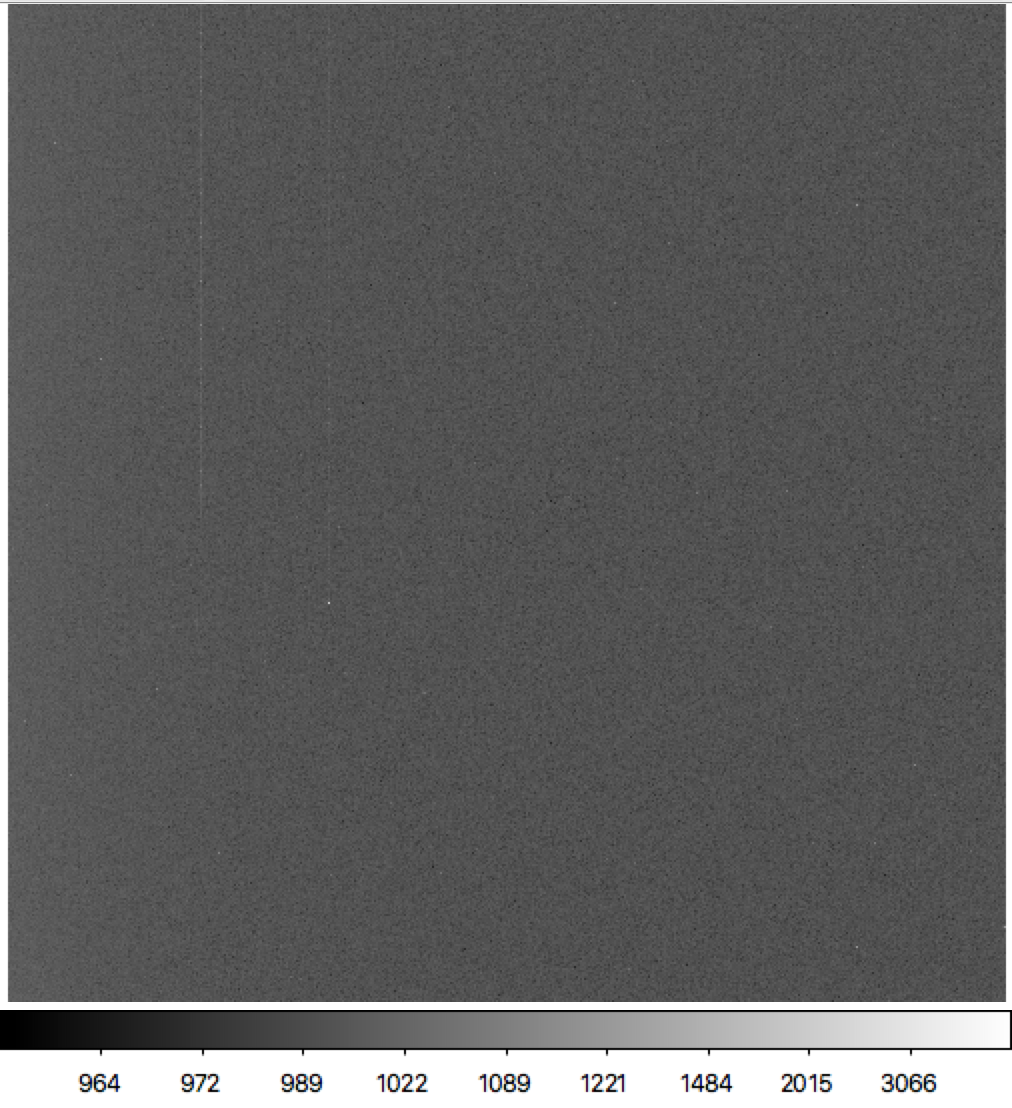
\includegraphics[width=3.5in]{../images/3p1_m10_00000000_BIAS.png}
    \caption{Bias frame}
    \label{fig:m10BIAS}
  \end{figure}

\section{Results and Conclusion}
I guess the bad pixel map and the resolution/dispersion of the spectrograph after it was all broken down.

\end{document}  